\section{Metodologia}

A atividade seguiu o procedimento proposto no roteiro \cite{Filter1}, dividindo-se nas etapas de síntese analítica, a definição da ordem do filtro, implementação do esquemático e validação computacional no ambiente \textit{Cadence Virtuoso} (ADE Maestro). Conforme as instruções especificadas, utilizaram-se componentes ideais das bibliotecas \texttt{analogLib} e \texttt{rfLib}, garantindo o casamento de impedância em $Z_0 = 50~\Omega$ nas portas de entrada e saída.


\subsection{Dimensionamento e Implementação Esquemática do Filtro}

Para o dimensionamento dos elementos, definiu-se primeiramente a frequência central de $f_0 = 6,5\text{ GHz}$ com largura de banda $BW = 500\text{ MHz}$, cuja motivação foi apresentada na Seção~\ref{sec:introducao}, seguindo as especificações estabelecidas no roteiro \cite{Filter1}.

Com base nos slides da aula \cite{schuartz2026slides}, a partir das informações contidas na Tabela~\ref{Tab:tabela1}, extraíram-se os coeficientes normalizados de quinta ordem ($N = 5$), resumidos na Tabela~\ref{tab:coeficientes_chebyshev}, para realizar os cálculos de dimensionamento dos componentes.

\begin{table}[htbp]
    \centering
    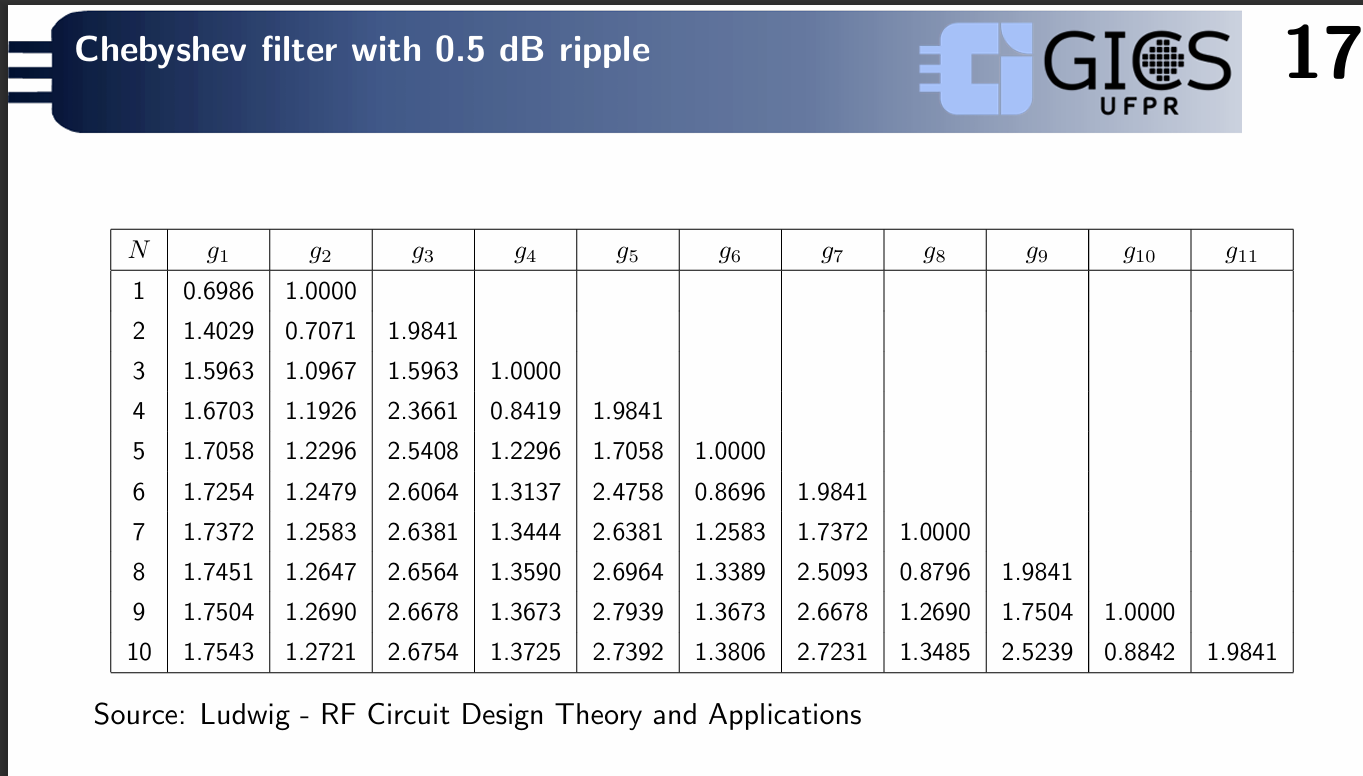
\includegraphics[width=\columnwidth]{Method/Fig/tabela1.png}
    \caption{Tabela de coeficientes normalizados para filtro Chebyshev com $0,5\text{ dB}$ de \textit{ripple} \cite{schuartz2026slides, ludwig2000rf}.}
    \label{Tab:tabela1}
\end{table}

\begin{table}[htbp]
    \centering
    \footnotesize
    \caption{Coeficientes normalizados do protótipo passa-baixas Chebyshev ($0,5\text{ dB}$ de \textit{ripple}, $N = 5$) \cite{ludwig2000rf, schuartz2026slides}.}
    \label{tab:coeficientes_chebyshev}
    \begin{tabular}{cccccc}
        \hline
        \textbf{$N$} & \textbf{$g_1$} & \textbf{$g_2$} & \textbf{$g_3$} & \textbf{$g_4$} & \textbf{$g_5$} \\
        \hline
        5 & $1,7058$ & $1,2296$ & $2,5408$ & $1,2296$ & $1,7058$ \\
        \hline
    \end{tabular}
\end{table}



Com valores obtidos na tabela \ref{tab:coeficientes_chebyshev}, foram realizado os calculos de dimensionamento para determinar os valore a seres atribuídos a cada componente:

\begin{align}
    f_L &= f_0 - \frac{BW_{\text{Hz}}}{2} = 6,25\text{ GHz} \\
    f_U &= f_0 + \frac{BW_{\text{Hz}}}{2} = 6,75\text{ GHz} \\
    \omega_0 &= 2\pi f_0 \approx 4,0841 \times 10^{10}\text{ rad/s} \\
    BW_{\text{rad}} &= 2\pi BW_{\text{Hz}} \approx 3,1416 \times 10^{9}\text{ rad/s}
\end{align}

Em seguida, realiza-se a desnormalização de impedância do protótipo passa-baixas para $R_G = 50~\Omega$, multiplicando os elementos indutivos ímpares ($g_1, g_3, g_5$) por $R_G$ e dividindo os elementos capacitivos pares ($g_2, g_4$) por $R_G$:
\begin{align}
    \tilde{L}_1 &= \tilde{L}_5 = g_1 R_G = 85,29\text{ H} \\
    \tilde{C}_2 &= \tilde{C}_4 = \frac{g_2}{R_G} = 24,592\text{ mF} \\
    \tilde{L}_3 &= g_3 R_G = 127,04\text{ H}
\end{align}

Por fim, aplica-se a transformação em frequência de passa-baixas para passa-faixa. Para os estágios série ($k = 1, 3, 5$), os valores dos indutores e capacitores são dados por:
\begin{align}
    L_1 &= L_5 = \frac{\tilde{L}_1}{BW_{\text{rad}}} = 27,15\text{ nH} \\
    C_1 &= C_5 = \frac{BW_{\text{rad}}}{\omega_0^2 \tilde{L}_1} = 22,08\text{ fF} \\
    L_3 &= \frac{\tilde{L}_3}{BW_{\text{rad}}} = 40,44\text{ nH} \\
    C_3 &= \frac{BW_{\text{rad}}}{\omega_0^2 \tilde{L}_3} = 14,83\text{ fF}
\end{align}

Para os estágios em paralelo (\textit{shunt}, $k = 2, 4$), os componentes ressonantes são obtidos por:
\begin{align}
    C_2 &= C_4 = \frac{\tilde{C}_2}{BW_{\text{rad}}} = 7,828\text{ pF} \\
    L_2 &= L_4 = \frac{BW_{\text{rad}}}{\omega_0^2 \tilde{C}_2} = 76,59\text{ pH}
\end{align}



Com os  valores dos componentes etao  resumidos na Tabela~\ref{tab:components}, 

\begin{table}[htbp]
    \centering
    \footnotesize
    \caption{Valores dimensionados dos componentes do filtro passa-faixa ($f_0 = 6,5\text{ GHz}$, $BW = 500\text{ MHz}$) e correspondência com o esquemático.}
    \label{tab:components}
    \begin{tabular}{cccc}
        \hline
        \textbf{Estágio ($k$)} & \textbf{Esquemático} & \textbf{Indutor} & \textbf{Capacitor} \\
        \hline
        1 (Série)    & \texttt{L0, C0} & $27,15\text{ nH}$ & $22,08\text{ fF}$ \\
        2 (Paralelo) & \texttt{L1, C1} & $76,59\text{ pH}$ & $7,828\text{ pF}$ \\
        3 (Série)    & \texttt{L2, C2} & $40,44\text{ nH}$ & $14,83\text{ fF}$ \\
        4 (Paralelo) & \texttt{L3, C3} & $76,59\text{ pH}$ & $7,828\text{ pF}$ \\
        5 (Série)    & \texttt{L4, C4} & $27,15\text{ nH}$ & $22,08\text{ fF}$ \\
        \hline
    \end{tabular}
\end{table}

 A modelagem do circuito do filtro foi implementada no \textit{Cadence Virtuoso}, conforme mostrado na Figura~\ref{fig:filtro_uwb_6g5}.


 \begin{figure}[htbp]
    \centering
    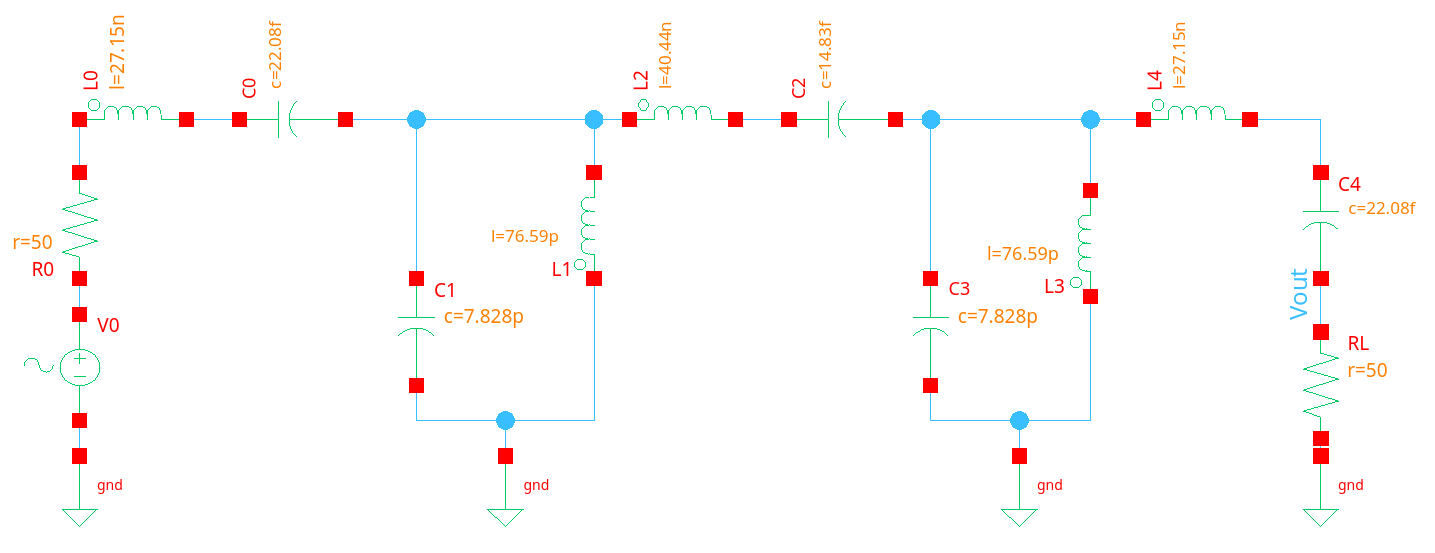
\includegraphics[width=\columnwidth]{Method/Fig/filtro_uwb_6g5.png}
    \caption{Esquemático do filtro passa-faixa UWB em $6,5\text{ GHz}$ implementado no \textit{Cadence Virtuoso}.}
    \label{fig:filtro_uwb_6g5}
\end{figure}